% Define the scope, extend, and how of the study
\chapter{Methodology}
\label{chap:methodology}

This chapter explains the methodology used in this study. 

The study is subdivided into four components, each representing a sub-research question, which is in turn based upon one of the challenges of a geo-web-vpl. 
The questions are posed in such a way that answering them will require us to explore the extend of this challenge, and find possible solutions.

(See reffig)

\begin{note}
TODO: diagram: 4 research questions -> four possible barriers of geocomputation
\end{note}

\begin{note}
TODO: diagram: show the 'locations' of the four research questions ( client / server / native, etc.)
\end{note}



\subsection*{Nature}
The methodology of this study can be characterized as practical as opposed to theoretical, 
% wholistic instead of specific, 
and iterative compared to linear. 
The prior works on browser-based geocomputation and geo-vpls indicate that a strong theoretical framework for a \ac{geo-web-vpl} is in place (Source). 
But, and this is especially evident in the prior studies regarding Browser-based geocomputation, the practical implementation of these theories were only partially successful, and limited in scope. 
This necessitates a practical approach in response. 
And, due to the investigative nature of this study, the methodology requires to iterate upon itself, instead of following a singular, linear path. 

% MIGHT NOW WANT TO KEEP THIS IN HERE

% ...
% % Theorie: is er maar je geloofde het niet
% % praktische implementatie om de Throerie weerleggen
% The prior works on browser-based geoprocessing indicate that a theoretical framework for browser-based geoprocessing vpl is in place. 
% But, and this is especially evident in the studies regarding client-side geoprocessing, the practical implementation of these theories

% Choices: 
% - practical > theoretical : Literature study indicates enough theoretical soundness, but lots of practical questions remaining. We wish to  immediate pick up where these studies have left, and therefore we choose the direct, practical study of designing and implementing a prototype application. 
% - wholistic > specific    : Research in one sub-domain could have been more exhaustive in one of the specific sub-studies, instead of covering the full scope it does now. However, This would have been incomplete. What we do now is cover the full pipeline of using a geocomputation library: from creation to web export, to web import, to web utilization. by doing this, we can identify issues caused in one of these
% - iterative > linear      : Given this vast scope, many questions can come up from different angles. The study has to be dynamic to adapt to these demands. 

\section{\mySubRQOneTitle} 
\label{sec:method-one}

The first component of the methodology involves the question of \mySubRQOneTitle : \mySubRQOne.

% [WHY]
Before exploring how lifting geo-computation to a web-VPL might take place, this study first wished to discover to what extend the web browser is able to facilitate the interface of a dataflow vpl for geometry computation in general, both in terms of data structures and visualization. 

The assumption that a geo-web-vpl should be implemented as a dataflow vpl is made because of the many advantageous qualities layed out in \refsec{sec:background:dataflow}. 
Additionally, and perhaps consequently, all comparable VPLs analyzed in \refsec{sec:related-geovpl} were implemented as dataflow VPLs (Blender, houdini, Grasshopper, GeoFlow), the only exception being the Möbius Modeller.
However, this meant that a new, web-based implementation had to be made, since no existing web-vpl concerned with geometry uses this model (that this study is aware of).

% As a second step, we wish to know to what extend a web-based, dataflow vpl can provide for the needs of a vpl meant for general 3D geometry processing.   
% A 3D VPL is defined as a vpl meant for generic 3D geometry processing.

% [HOW]
The following approach was deemed as the most fitting method to answer this question of \mySubRQOneTitle:
\begin{enumerate}[A]
  \item \emph{Define the requirements of a dataflow-VPL handling geometry}
  \item \emph{Define 'core browser features'}
  \item \emph{Implement a dataflow-VPL in a browser according to these features}
  \item \emph{Per requirement, to what extend is it successfully implemented by this dataflow-VPL?}.
  \item \emph{Per requirement, which role did the core browser features play in supporting or hindering it?}.
  % \item \emph{Per implemented requirement, to what extend does this web implementation differ from native dataflow VPLs?}
\end{enumerate}

The definitions for step A and B will be made subsequently. 
The implementation of step C is presented at \refsec{sec:implementation:representation}, 
and the assessments of D and E can be found in \refsec{sec:analyses:representation}

\subsection*{A: Requirements}

The requirements of a dataflow-VPL implementation can be subdivided in requirements of a dataflow VPl in general, and a VPL for geo-computation specifically.
Based on (SOURCE: dataflow VPL) any dataflow-VPL must at the very least contain the following aspects: 
\begin{enumerate}[-]
  \item a base 'programming language model'
  \subitem A representation of the 'variables' and 'functions' of the language
  \subitem With all computations being pure functions
  \subitem With all variables being immutable
  \item a 'graph-like' visualization of this data model
  \item an interface to create and edit this graph 
  \item a way to provide input data 
  \item a way to execute the language
  \item a way to display or save output data
\end{enumerate}
The implementation of these aspects would result in a 'baseline', general purpose, dataflow VPL. 
To specialize this implementation further, A visual programming language handling geometry should have:
\begin{enumerate}[-]
  \item Type safety 
  \item A way to load or to create geometry data 
  \item A way to export geometry data
  \item A method to preview geometry data in 3D
  \item A standard set of geometric types and operations
\end{enumerate}
These requirements need further explanation.
First, regarding type safety.
In this context, type safety refers to: 
The input and output of a function should have a type stated, and users should be notified of incorrect usage of types, or 'invalid connections'.
Geometry VPLs in particular need this, as many data representations of geometry are required to be precise about their data usage.
A VPL used to construct geometry should reflect this. 
Similarly, it should be possible to define these geometry representations as inputs, or to extract them as output. 
This will require specialized parsers to become part of the VPL. 
Additionally, when these types are clear and clearly communicated, users must have ways to provide these types as inputs or outputs. 

Regarding visualization, A hallmark of dataflow VPLs is the ability to inspect the geometry created in in-between steps, so this must be provided for.
This is also a good fit, since the immutable nature of dataflow VPL variables make these variables ideal for caching. 

Finally, a geometry VPL should contain a set of 'internal', basic types and operations.
All aforementioned features are difficult to implement without defining some set of internally recognized data types. 
Basic operations are needed in particular to transform between the types.

% \begin{note}
%   Figure out what to do with this: 
%     Interactivity is the defining factor of the vpl. 
%     a list of standard VPL features & application features required as a base-line:  
%   - Users must be able to construct a script by visual means.

\subsection*{B: Core browser features}

\begin{figure}
  \centering
  \graphicspath{ {../../assets/plots/browser-usage/} }
  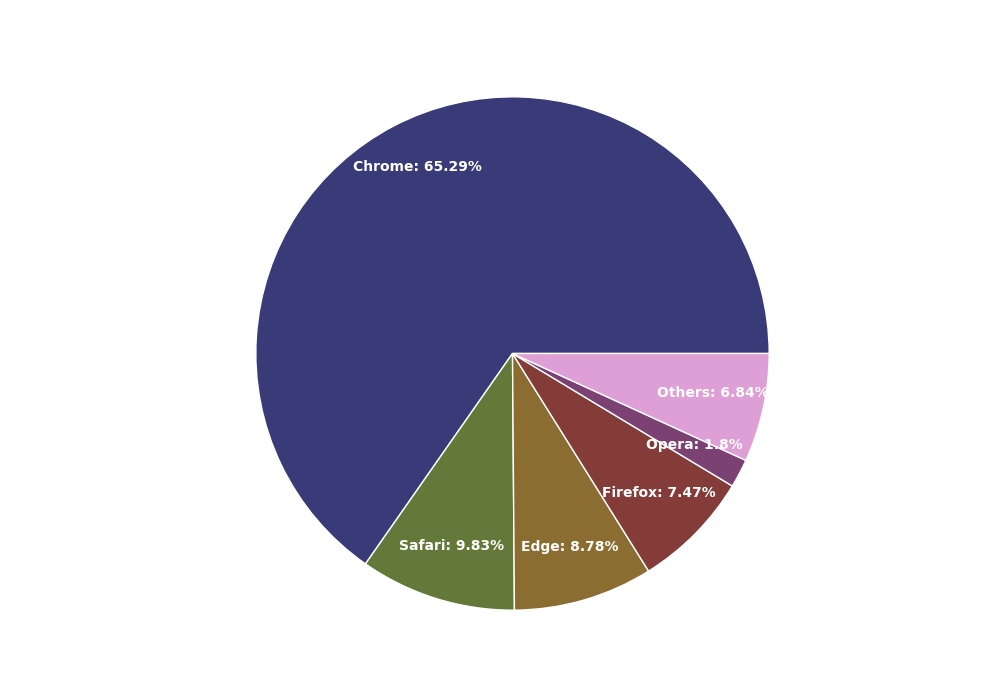
\includegraphics[width=0.7\linewidth]{plot.png}
  \caption[Browser usage]{Fall 2021 desktop browser usage statistics. Data averaged over (Source, Source, Source, and Source)}
  \label{fig:browser-usage}
\end{figure}

This study defines "Core browser features" as the set of default features implemented by the browser engines of 'major browsers'. 
Based on the desktop browser market shares of \reffig{fig:browser-usage}, the chromium based browsers (Chrome, Edge, Opera) have the majority. 
This is followed up by Firefox, based on the Gecko engine, and Safari, based on webkit. 
By supporting these three engines, the vast majority of end-users can be accounted for. 

The set of features common in these three browser engines are well-documented on websites like MDN web docs (SOURCE: Mozilla). 
This set includes the following features relevant for the 3D VPL:
\begin{enumerate}[-]
  \item WebGL \& WebGL2 (WebGPU is not fully covered yet)
  \item 2D Canvas API
  \item Web Workers
  \item Web Components
  \item WebAssembly
\end{enumerate}

% \subsection*{C: Implementation Steps}

% \begin{note}
% TODO: An image showing the phases of development
% \end{note}

% To find the answer to question C, this study implemented the core of the prototype \ac{geo-web-vpl}.
% Just like the entire study, the development trajectory for implementing will be done incrementally, ensuring results during all steps of the development. 
% The first step of the phase consists of creating the basics of the \ac{gui} itself. 
% A basic \ac{vpl} will be created which can only process boolean statements. 
% The second step involves developing the main datamodel of the VPL, to represent the program in an object-oriented way. 
% The third step adds types, geometry, and the visualization of this geometry in 3D, as well as textures / images in 2d. \
% The fourth step adds geospatial data support, and adds Web Feature Services, Web Map Services, and coordinate reference systems.  

%%%%%%%%%%%%%%%%%%%%%%%%%%%%%%%%%%%%%%%%%%%%%%%%%%%%%%%%%%%%%%%%%%%%%%%%%%%%%%%%%%%%%%%%%%%%%%%%%%%%%%%%%%%%%%
%%%%%%%%%%%%%%%%%%%%%%%%%%%%%%%%%%%%%%%%%%%%%%%%%%%%%%%%%%%%%%%%%%%%%%%%%%%%%%%%%%%%%%%%%%%%%%%%%%%%%%%%%%%%%%
%%%%%%%%%%%%%%%%%%%%%%%%%%%%%%%%%%%%%%%%%%%%%%%%%%%%%%%%%%%%%%%%%%%%%%%%%%%%%%%%%%%%%%%%%%%%%%%%%%%%%%%%%%%%%%
%%%%%%%%%%%%%%%%%%%%%%%%%%%%%%%%%%%%%%%%%%%%%%%%%%%%%%%%%%%%%%%%%%%%%%%%%%%%%%%%%%%%%%%%%%%%%%%%%%%%%%%%%%%%%%
%%%%%%%%%%%%%%%%%%%%%%%%%%%%%%%%%%%%%%%%%%%%%%%%%%%%%%%%%%%%%%%%%%%%%%%%%%%%%%%%%%%%%%%%%%%%%%%%%%%%%%%%%%%%%%

\section{\mySubRQTwoTitle} 
\label{sec:method-two}
The second component of the methodology seeks an answer to the question of \mySubRQTwoTitle: \mySubRQTwo

\begin{note}
  REQUIREMENT: libraries containing pure functions exclusively
  - no side effects, thats the whole point  
\end{note}


% [Why]
Making sure a \ac{geo-web-vpl} is able to make use of native, system-level libraries is a key component, since it will mean access to powerful, industry standard geocomputation libraries like CGAL and GDAL. 
The most viable option for using a non-js library in a web browser, is by compiling it to WebAssembly \cite{haas_bringing_2017}.
Other options exist, like simply rewriting non-js languages to JavaScript, but these methods have significant drawbacks \cite{haas_bringing_2017,jangda_not_2019}.
However, as described in \refsec{sec:related-geoweb} compiling libraries to \ac{wasm} also may pose challenges:

% The study starts out with the assumption that WebAssembly must be utilized to properly compile and run existing geoprocessing libraries in a browser. This might not be as easy as using normal compilers, based on the experience gained by preliminary work (See \autoref{sec:preliminary-wasm}). WebAssembly is containerized and makes no assumptions about its source language \cite{haas_bringing_2017}, making aspects such as an SDK, sub-dependencies called using environment variables, and IO (file reading and writing) possible obstacles. 

\begin{enumerate}[-]
  \item \ac{wasm} promises a 'near native performance' (Source: Wasm). However, this can be quite situational, as multiple studies have shown \cite{jangda_not_2019} (Source: the bachelor thesis). 
  \item \ac{wasm} cannot compile all code. Its containerized nature means that code accessing a file system for example, does not function without workarounds. 
  \item Compiled \ac{wasm} code could be difficult to access and interface in a web browser. Without third-party tools, functions exposed by \ac{wasm} can only accept primitive data types as input. There is no \m{string} data type, let alone a \m{struct} or \m{object} type. 
  \item Compiling an \emph{library} to \ac{wasm} is seriously different from compiling a full \emph{application} to wasm. A library requires more complicated wasm-javascript interoperability, which third-party tools may or may not be able to provide.
\end{enumerate}
Discovering the extend and relevance of these compilation challenges for geo-computation libraries is why the sub-question of \mySubRQTwoTitle \space was included in this study. 

% [HOW]
Two experiments are conduced to answer this supporting research question. 
The first focusses on making a clear, measurable comparison between compilation methods, where the second experiment focusses on compilation in a practical, realistic scenario. 

Both studies limit themselves to native libraries written in C++ and Rust. 
C++ was chosen, since almost all relevant geocomputation libraries are written in C++, like CGAL and PROJ. 
Rust was chosen, since this language is likely to be a future choice for geocomputation libraries, and possesses powerful WebAssembly support. 

%%%%%%%%%%%%%%%%%%%%%%%%%%%%%%%%%%%%%%%%%%%%%%%%%%%%%%%%%%%%%%%%%%%%%%%%%%%%%%%

\subsection{First Experiment}
The first experiment compares three different methods of bringing the same geocomputation procedure to the web. 
This way, quantitative, measurable aspects of these methods can be compared. 
The following three methods are tested:
\begin{enumerate}[-]
  \item Write the procedure in normal javascript
  \item Write the procedure in C++, compile to wasm using the \m{emscriptem} toolkit (Source)
  \item Write the procedure in Rust, compile to wasm using the \m{wasm-bindgen} toolkit (Source)
\end{enumerate}
These procedures are all tested within the same web application, using the same data. 
By taking two different languages, we can distinguish between shortcomings of \ac{wasm} itself, and the \ac{wasm} support of a language.  

The procedure chosen is a 2D convex hull calculation of a set of sample points. 
The chosen procedure must be small enough to clearly reason about performance differences, and yet large enough to pose a substantial computational challenge, validating the usage of \ac{wasm}.

\begin{note}
  Expand upon the procedure
\end{note}

The three methods will be compared in terms of:
\begin{enumerate}[-]
  \item performance
  \item load times
  \item memory usage
\end{enumerate}

\begin{note}
  - todo: turn features around into assessment criteria
  - performance: load times, run times
  - current state of webassembly & js. how much faster is it? is it even faster? 
     - data translation steps, do they mitigate performance gains? 
     - also given the fact that we are doing 'functions on sets'/ declarative instead of imperative styles, forced by the format of dataflow programming. 
\end{note}

The studies on browser-based geocomputation (\refsec{sec:related-geoweb}) appear to have conducted a similar experiment, by comparing the same procedure written in C++ and javascript. 
However, these studies compared javascript against a native, non-web compilation of C++. 
This experiment also differs in distinguishing between \ac{wasm} itself, and a language's \ac{wasm} support.

%%%%%%%%%%%%%%%%%%%%%%%%%%%%%%%%%%%%%%%%%%%%%%%%%%%%%%%%%%%%%%%%%%%%%%%%%%%%%%%

\subsection{Second Experiment}
The second experiment is a qualitative comparison between compiling a full-scale library written in Rust, to a full library written in C++. 
This way, the tooling and workflow can be compared for a realistic use-case. 
The study will be conducted by attempting to compile both libraries using their respective \ac{wasm} toolsets, and noting the differences in workflow, supported features, and the resulting wasm library. 

we wish to compile these languages without 'disturbing' them: they must be kept the exact same for normal, native usage. 
We will instead create 'wrapper' libraries. 

\subsubsection*{Library One: CGAL}
The first library tested is CGAL, written in C++, compiled using \m{emscriptem}.
CGAL will be used as an exemplary C++ library. 
For one, this library is well established and very relevant to geoprocessing as a whole. 
Many other C++ geo-libraries depend on it.
Moreover, it is a sizable and complex project, making it highly likely the problems described by related works will be encountered. 
We could choose more simple libraries, but this will not be representative of most C++ geoprocessing libraries. 

\subsubsection*{Library Two: Startin}
The second library tested is the Startin library, written in Rust, compiled using \m{wasm-bindgen}.  
This library is both smaller in scope, and less well-known than CGAL. 
Ideally, a library with a size and popularity comparable to CGAL should have been chosen.
However, Rust is still a relatively unknown language in the field of GIS. 
Startin was chosen, for the triangulation functionalities it provides are comparable to that of CGAL, in terms of performance, and geometric robustness (Source). 

%%%%%%%%%%%%%%%%%%%%%%%%%%%%%%%%%%%%%%%%%%%%%%%%%%%%%%%%%%%%%%%%%%%%%%%%%%%%%%%

\section{\mySubRQThreeTitle} 
\label{sec:method-three}

In this third component of the methodology, we wish to discover how the web-exposed geocomputation libraries of \refsec{sec:method-two} can be utilized within the 3D VPL of \refsec{sec:method-one}. 
This is once more a crucial aspect for the success of the entire \ac*{geo-web-vpl}, 
and captured by the research question: \mySubRQThree

% to what extend can a web-consumable library be loaded into a web-vpl without explicit configuration?

% [Why]

\begin{figure}
  \centering
  \graphicspath{ {../../assets/images/4/} }
  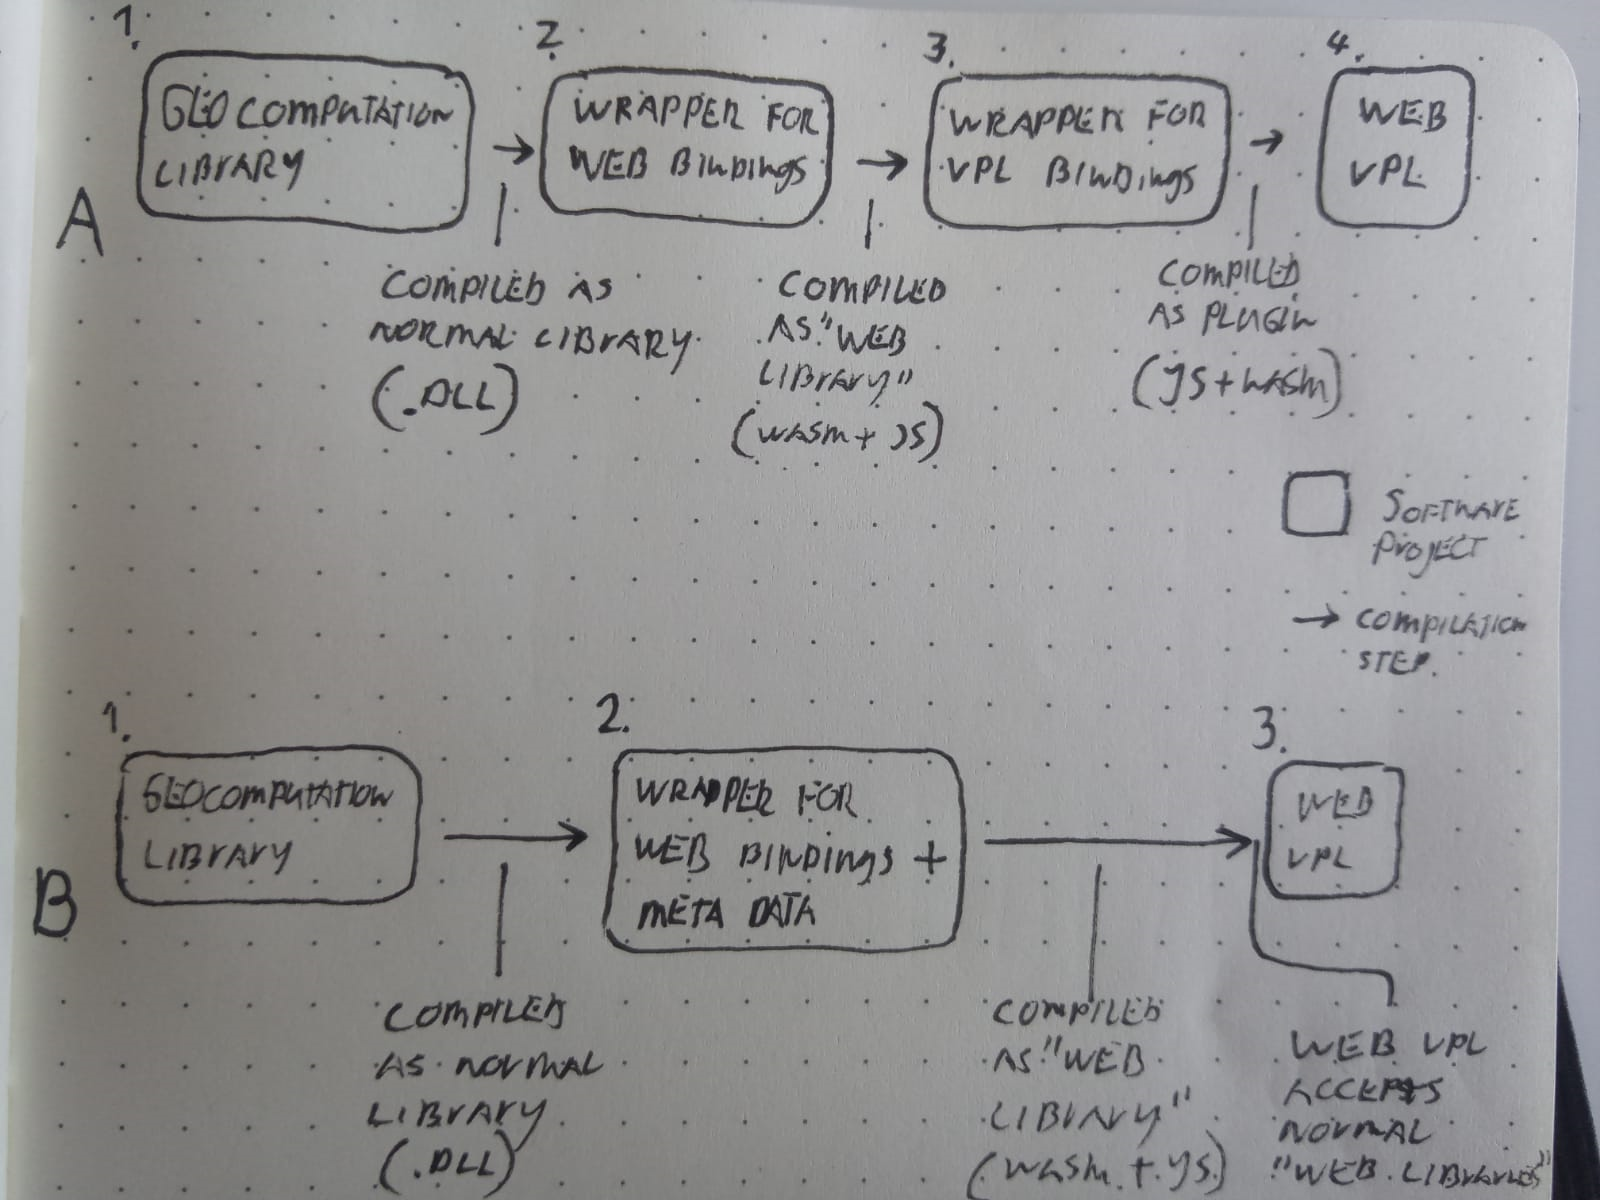
\includegraphics[width=\linewidth]{loading-trajectory.png}
  \caption[Loading Trajectory]{Loading Trajectories}
  \label{fig:loading-trajectory}
\end{figure}

% THE REASON FOR THIS WAS DISCOVERED DURING PRELIMINARY STUDIES

Most of the 3D vpls mentioned in \refsec{sec:background-vpl} offer a plugin system, or some other way to load external libraries.
This way, the functionalities of the environments can be expanded upon.
However, all of these plugin / library systems require explicit 'wrapper' libraries, to explain how the functionalities a text-based programming library map to components used in a visual manner.
This turned out to be a problem during preliminary studies.
If a \ac{geo-web-vpl} wishes to use non-js libraries, it would mean that these libraries would have to be wrapped twice (see \reffig{fig:loading-trajectory} A): 
Once to expose the native library to the web using the methods described at \refsec{sec:method-two},
And once more to map the web library to the visual language. 
While this is a possibility, in practice, two layers of indirection are not acceptable in terms of a development workflow.
This would be cumbersome, prone to errors, and hurting version control by having to synchronize between 4 software projects. 

There is also a second reason for critically addressing the way plugins are loaded. 
An observation was made from studying the existing geo-vpls in \refsec{sec:related-geovpl}:
It seems that if a developer wants to create custom VPL components, they are required to write plugins very specific to that particular VPL.
This means that practically, the library ecosystem of a VPL is entirely its own: 
It is separated from the wider context of textual programming libraries. 
End users are at the mercy of developers implementing their libraries in the dialect their particular VPL.
Meanwhile, developers are forced to implement and support a multitude of wrapper libraries for VPL platforms.  

In contrast, if the library loader of a VPL was able to directly utilize textual libraries, the barrier between vpl ecosystems and regular text-based libraries would cease to exist, benefiting both developers and end users. 
It might even lower the barrier between visual and textual programming in general, making it easier for VPl end-users to adopt some forms of textual programming, and vice versa. 

These two reasons are why this third component of the methodology is focused on exploring and assessing a method to  mitigate the need for the second wrapper library. 
The following plan was used: 
\begin{enumerate}[-]
  \item Design a library / plugin model for the prototype \ac*{geo-web-vpl}
  \item Implement this library model 
  \item Assess to what extend it mitigates the need for explicit configuration
  \item Assess to what extend this creates seamless interoperability between textual programming libraries, and VPL libraries.
\end{enumerate}

The design is given subsequently, the build implementation and assessment can be found in \refsec{sec:implementation:loading} and \refsec{sec:analyses:loading}.

\subsection{Design \& Method}

\begin{note}
 TODO: I should elaborate the design some more
\end{note}

The library model consists of two components: the design for a geo-web-vpl library, 
and the design for a loader on the side of the VPL. 
The central idea for this model is to take the wasm-wrappers created in \refsec{sec:method-two}, and to either interpret the required information from the wasm binary and related files, or, if that is impossible, add the required information in the wasm wrapper library itself as meta data.
By doing so, we make sure that at the very least, only one wrapper library is required for exposing any non-js library to the \ac{geo-web-vpl}.
The following information is required for the VPL to load a geocomputation library, and convert it into visual components:
\begin{enumerate}[-]
  \item A list of all functions present in the library, named.
  \item A list of all custom types (structs / classes) present in the library, also named.
  \item Per function:  
  \subitem A list of all input parameters, name and type.
  \subitem An output type.
\end{enumerate}

The following information is optional, but it would aid the functionality and usability of the library tremendously:
\begin{enumerate}[-]
  \item Per function:
  \subitem A custom, human-readable name.
  \subitem A description to explain usage.

  \item Per type:
  \subitem A custom, human-readable name.
  \subitem A description to explain usage.
  \subitem A definition of how to serialize and deserialize this type  
  \subitem A definition of how to render this type in 2D or 3D
  \subitem A definition of how to convert this type to basic types present within the geo-web-vpl.  
\end{enumerate}

The necessity to automate loading geocomputation libraries means that the \ac{geo-web-vpl} needs to be able to extract this information automatically. 

%%%%%%%%%%%%%%%%%%%%%%%%%%%%%%%%%%%%%%%%%%%%%%%%%%%%%%%%%%%%%%%%%%%%%%%%%%%%%%%
%%%%%%%%%%%%%%%%%%%%%%%%%%%%%%%%%%%%%%%%%%%%%%%%%%%%%%%%%%%%%%%%%%%%%%%%%%%%%%%
%%%%%%%%%%%%%%%%%%%%%%%%%%%%%%%%%%%%%%%%%%%%%%%%%%%%%%%%%%%%%%%%%%%%%%%%%%%%%%%
%%%%%%%%%%%%%%%%%%%%%%%%%%%%%%%%%%%%%%%%%%%%%%%%%%%%%%%%%%%%%%%%%%%%%%%%%%%%%%%
%%%%%%%%%%%%%%%%%%%%%%%%%%%%%%%%%%%%%%%%%%%%%%%%%%%%%%%%%%%%%%%%%%%%%%%%%%%%%%%

\section{\mySubRQFourTitle} 
\label{sec:method-four}

\begin{note}
  CUT OUT THE USE-CASE APPLICATION ASPECT. 
  -> we can make a utilization assessment based on the criteria alone, We dont need to create an application.
\end{note}

The final component of the methodology is dedicated to overcoming the fourth and final challenge to realizing a \ac{geo-web-vpl}, and involves the utilization of all aforementioned components. 
In this section, we wish to discover the practical usefulness of a \ac{geo-web-vpl}, encompassed by the research question : \mySubRQFour

% What are the advantages and disadvantages of using an existing geoprocessing library through a geo-web-vpl, as opposed to native utilization of said library?

% [WHY]
This component of the methodology is included in the study because of the following: 
It might be the case that a geo-web-vpl \emph{is} able to represented by a web-browser, and \emph{is} able to load and run functions from native, non-js geo-computation libraries. 
And still, it might not be able to successfully \emph{use} these libraries. 
The entire idea of a vpl might not be sensible for the operation at hand, or some other, unforeseen aspects mitigates the practical usefulness of the environment. 
It is therefore vital to access the actual usage of the application for accessing a geocomputation library.

% [HOW]
To answer the question of \mySubRQFourTitle, the various applications created within Geofront will be subjected to a qualitative assessment. 

% \begin{enumerate}[-]
%   \item Develop a representative use-case application within the prototype \ac{geo-web-vpl}.
%   \item Develop a command line application capable of the very same process.
%   \item Assess both applications according to a series of assessment questions.
% \end{enumerate}

% The execution of this component of the methodology is found in \refsec{sec:analyses:utilization}.

% \subsection{use-case application}
% The application used in both test cases is an "isocurves from DTM" process. 
% But also: we want the iso-curves of a specific location. How to get this data is part of the exercise

% \begin{note}
% [This is subject to change, according to how much I can accomplish ]

% - find the required height data as WFS / WMS
% - determine a boundary
% - load a dtm as a regular png / tiff image
% - specify the parameters, like height delta, smoothness.
% - marching squares
% - post-process curves
% - save as wkt, geojson, or some other well-known vector format

% \end{note}

\subsection{Assessment Framework}
For the assessment criteria, the cognitive dimensions framework of \cite[]{green_usability_1996} will be used. 
The framework is useful for its focus on language features. 
This allows the assessment to be made within the scope of this study, and without performing user-testing.
Also, as commented on in \refsec{sec:background-vpl}, the study has acquired a canonical nature among many VPL researchers for its elaborate examination of the "Psychology of Programming".
The age of the study indicates that the principles have stood the test of time. 

The framework presents the following 13 dimensions and accompanying descriptions \cite[]{green_usability_1996}:
\begin{enumerate}
  \item Abstraction gradient: What are the minimum and maximum levels of abstraction? Can fragments be encapsulated? 

  \item Closeness of mapping: What 'programming games' need to be learned? 
  
  \item Consistency: When some of the language has been learnt, how much of the rest can be inferred? 
  
  \item Diffuseness: How many symbols or graphic entities are required to express a meaning? 
  
  \item Error- proneness: Does the design of the notation induce 'careless mistakes'? 
  
  \item Hard mental operations: Are there places where the user needs to resort to fingers or pencilled annotation to keep track of what's happening? 
  
  \item Hidden dependencies: Is every dependency overtly indicated in both directions? Is the indication perceptual or only symbolic? 
  
  \item Premature commitment: Do programmers have to make decisions before they have the information they need? 
  
  \item Progressive evaluation: Can a partially-complete program be executed to obtain feedback on 'How am I doing'? 
  
  \item Role- expressiveness: Can the reader see how each component of a program relates to the whole? 
  
  \item Secondary notation: Can programmers use layout, colour, other cues to convey extra meaning, above and beyond the 'official' semantics of the language? 
  
  \item Viscosity: How much effort is required to perform a single change? 
  
  \item Visibility: Is every part of the code simultaneously visible (assuming a large enough display), or it it at least possible to juxtapose any two parts side-by-side at will? If the code is dispersed, is it at least possible to know in what order to read it?
\end{enumerate}

As stated by the authors; the purpose of this framework is to make the trade-offs chosen by a language's designer explicit. It is not meant as a 'scoring' system.

% Nielsen and Molichs 10 User Interface Design Guidelines
% https://theomandel.com/resources/golden-rules-of-user-interface-design/
% https://www.interaction-design.org/literature/article/user-interface-design-guidelines-10-rules-of-thumb
% (old rules, but still relevant)_

